\chapter{Adaptive Strategy for Iterative Join Execution}
\label{sec:adapt}

The most resource-intensive task of answering a SPARQL query is to perform the graph pattern matching over the RDF dataset. 
The graph matching operator executes a series of join operations between RDF triples that matches the triple patterns. Join operations have the greatest impact on the overall performance of a SPARQL query engine, typically requiring a large number of comparison operations that can only be done efficiently if records are stored in memory. 

\section{Join Propagation Algorithms}

The join performance can be tuned by optimisation algorithms which plan optimal join orders and join algorithms~\cite{Stocker:2008,Neumann:2008,Tsialiamanis:2012}. 
These approaches assume that memory is always available during the course of the execution of a chosen query plan. However, in  light-weight computing devices memory is critically low and, as such, the memory resource available for an RDF engine is unreliable, e.g. a surge of number network connections to the device might drain out available memory for all other running processes. Lack of memory may block  join operations that require temporary virtual memory such as hash-joins or sorted-merge joins,  and thus hurts the overall performance of the query engine or probably crashes the engine.

Materialisation techniques that write intermediate join results to storage is an attractive solution for the issue of  memory shortage~\cite{Garcia-Molina:2008}. However, on flash storage, writing is much slower if a random write happens. Furthermore, a limited number of erase operations can be applied to a block of flash memory before it becomes unreliable. 

To minimise the memory required  to execute a SPARQL query making the best usage of the indexing scheme introduced in Section~\ref{sec:index}, we adopt the \textit{one-tuple-at-a-time} paradigm to compute the join. This approach can reduce the memory consumption as no virtual temporary memory is required to buffer the intermediate join results. 
The basic idea of the algorithm to compute the join of a graph pattern is as follows.
A mapping solution (mapping for short) is continuously sent to visit each triple pattern of the graph pattern.
In each visit, it searches for triples matching with the triple pattern.
For each matched triple, variables in the triple pattern and the corresponding value in the triple are added to the mapping.
The mapping with new values will be sent to visit the next triple pattern, or be returned as query result when all triple patterns have been visited.

%===================================================================================================
\begin{algorithm}[ht!]
\label{alg:jp}
\caption{Join propagation}
	\SetKwProg{Fn}{Function}{}{end}
	\SetKwFunction{fn}{findNextPattern}
    \SetKwFunction{eval}{eval}
    \SetKwFunction{bind}{bindMapping}
    \SetKwFunction{reset}{resetMapping}
    \SetKwFunction{isCompatible}{isCompatible}
    \SetKwFunction{jp}{propagate}
    \SetKwInOut{Input}{input}
    \SetKwInOut{Output}{output}
     
    \Fn{\jp{$\mu$, $\mathbb{P}$}}
    
    \Input{$\mu$        : mapping, 
           $\mathbb{P}$ : set of triple query patterns}
           
    \Output{$\mu$ : mapping} 
    
    \If {isEmpty($\mathbb{P}$)}
    {
      	\Return $\mu$;
    }
    
    $p    \leftarrow$ \fn{$\mu, \mathbb{P}$}\;
    $p_{key}     \leftarrow  createKey(\mu, p)$\;
	$\mathbb{T}  \leftarrow$ indexScan($p_{key}$)\;
    $\mathbb{P}' \leftarrow$ $\mathbb{P}\setminus\{p\}$\;
    
    \For{$t$ $\in$ $\mathbb{T}$}
    {
    	$\mu$ $\leftarrow$ \bind{t, $p$}\;
      	\jp{$\mu$,  $\mathbb{P}'$}\;
        $\mu$ $\leftarrow$ \reset{t, $p$}\;
    }
\end{algorithm}
%=================================================================================================================


The abstract of the join propagation algorithm is given in the Algorithm 1. The propagate($\mu$, $\mathbb{P}$) function  is used to recursively propagate the input mapping. 
The function starts with an empty mapping $\mu$ and a set of unvisited triple patterns $\mathbb{P}$.
For each run, it checks and returns the input mapping as a result if there is no triple pattern left to visit (line 1-2). Based on the given input mapping, it looks for the optimal unvisited triple query pattern to visit (line 3). 
To search for triples compatible with pattern p, an index search key $p_{key}$ is created by replacing the variables in p according to $\mu$ (line 4). 
For each matched triple \textit{t}, the corresponding variables and values are bound into the mapping. Then another propagation of the mapping to the remaining unvisited triple patterns is called (line 7-10).

In each run of the propagation algorithm, the function findNextPattern($\mu$, $\mathbb{P}$) is called to find the optimal triple pattern to execute the propagation (see Function 1).
For each triple pattern \textit{p} in $\mathbb{P}$, the set of triple query patterns , the function searches for a triple pattern that shares variables with the input mapping $\mu$ at line 4. With each shared pattern found, an index search key pattern, $p_{key}$, is created (line 5). An index lookup on  $p_{key}$ is executed to search for the upper bound and lower bound positions of the set of the matching triples in the index, as described in the previous section (line 6). The size of the index lookup $\mathbb{I}$ is defined as the range between the upper bound and  lower bound positions (lined 7-9). The function returns the triple pattern that has the minimal size of the index lookup at line 11.


\section{Routing Policy}

%================================================================================================================================
\begin{function}[ht!]
\caption{1: findNextPattern($\mu, \mathbb{P}$)}
\SetKwProg{Fn}{Function}{}{end}
    \SetKwFunction{findNextPattern}{findNextPattern}
    \SetKwInOut{Input}{input}
    \SetKwInOut{Output}{output}
     
    %\Fn{\findNextPattern{$\mu$, $\mathbb{P}$}}
    
    \Input{$\mu$ : mapping, $\mathbb{P}$ : set of triple query patterns}
    \Output{P : triple query pattern} 
    
    $p_{next}\leftarrow null$\;
    $s_{min}\leftarrow Integer_{max}$\;
    
    \For{p $\in$ $\mathbb{P}$}
    {
      \If{isShared($\mu$, p)}
      {
		$p_{key} \leftarrow  createKey(\mu, p)$\;
        $I       \leftarrow  indexLookUp(p_{key})$\;
        $s       \leftarrow  sizeOf(I)$\;
        
        \If{$s < s_{min}$}
        {
           $s_{min}\leftarrow s$\;
           $p_{next}\leftarrow p$\;
        } 
      }
    }
    \Return $p_{next}$\;
\end{function}
%================================================================================================================================

The join propagation algorithm is similar to the nested iterations. Nested loop join is often argued to give poor performance as it does not attempt to prune the number of comparisons. However, equipped with an efficient index scheme, an index nested loops join can perform as well as other join algorithms~\cite{Graefe:2003}.
With the design of our storage, the index lookup can be done mostly within the buffer layer, only two extra I/Os may be required. The visitor pattern, that sends a mapping to visit each triple pattern and to execute index lookup, reduces the extra memory for the joins as only a mapping is kept in the main memory. This mechanism also enables the adaptivity for the joins. The function findNextPattern($\mu, \mathbb{P}$) decides which triple pattern the mapping should visit first. Similarly to routing policy of the stream processing engines, e.g Eddies~\cite{Avnur:2000} or CQELS~\cite{Danh:2011}, this function defines the propagating policy to achieve a certain optimisation purpose. In our case, we attempt to minimise the number of the propagations by choosing the shortest index scan in each run. Note that, this is the key place holder to add sophisticated optimisation algorithms, e.g. adaptive caching algorithm to be discussed in our future work.  

\section{Cost model}

\section{Evaluation}


\begin{figure}[ht!]
\centering
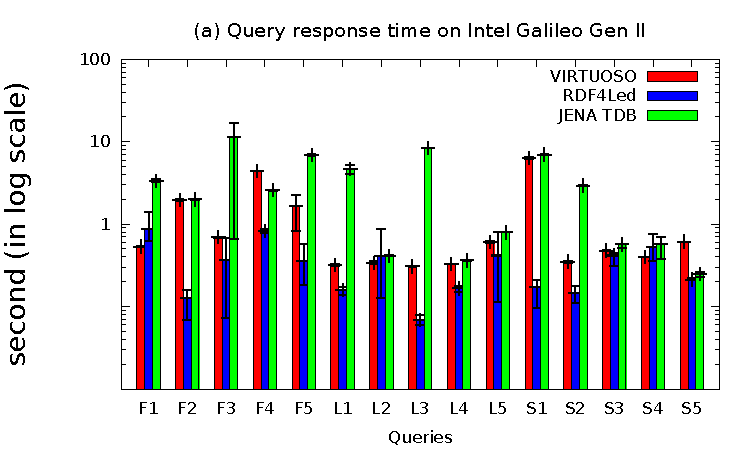
\includegraphics[width=0.3\textwidth]{c6/GII_QUERY_WATDIV_20.pdf}
\label{fig:result_query}
\end{figure}

\begin{figure}[ht!]
\centering
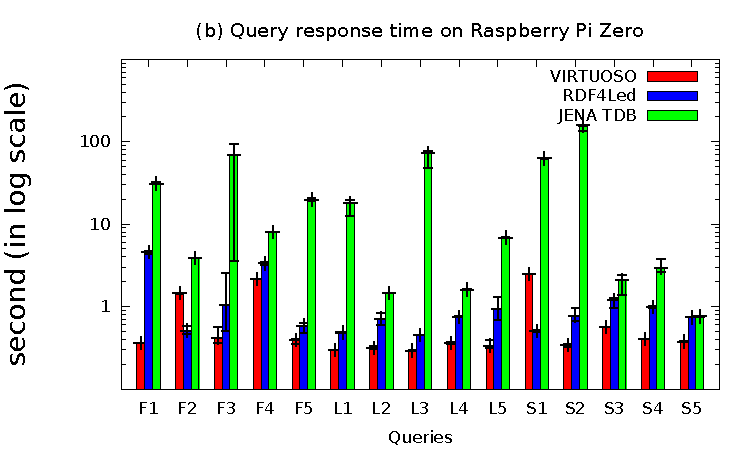
\includegraphics[width=0.3\textwidth]{c6/PI0_QUERY_WATDIV_100.pdf}
\label{fig:result_query}
\end{figure}

\begin{figure}[ht!]
\centering
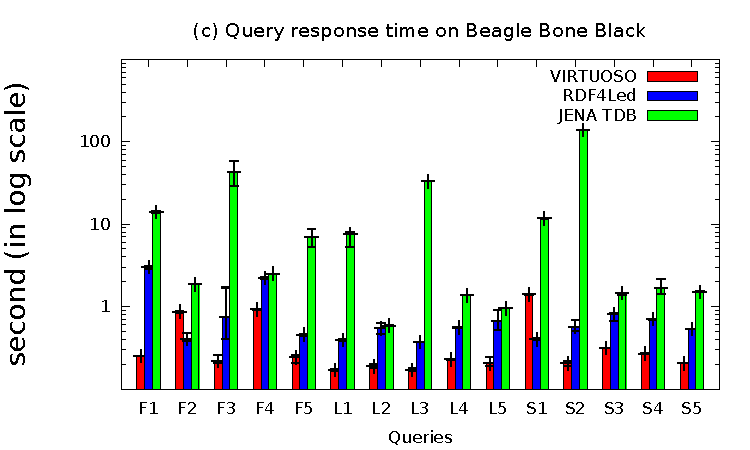
\includegraphics[width=0.3\textwidth]{c6/BBB_QUERY_WATDIV_100.pdf}
\label{fig:result_query}
\end{figure}

On all the devices, RDF4Led answered all the queries considerably faster than Jena TDB did. Both RDF4Led and JenaTDB follow the nested execution model to compute the multiple joins between RDF triples that match triple patterns. However, Jena TDB was implemented with iterator pattern, while RDF4Led followed the visitor pattern. In general, both algorithms execute lookup operations and index scan operations to extract the compatible triples from the dataset. The performance of these algorithms is mainly influenced by the performance of the lookup and index scan operations on the indexes. The better performance of RDF4Led against Jena TDB explains that our lightweight index structure helps RDF4Led outperform the B$+$ tree implemented in Jena TDB.  

\vspace{-1.5mm}
With the same dataset and on the same device, RDF4Led only answered the queries generated from templates F2 and S1 faster than Virtuoso does. These queries contain the graph patterns which have more than 6 triple patterns that form a star shape. In other cases, RDF4Led was slower than Virtuoso as it did not aggressively pre-allocate a fixed amount of memory (2-3 times more) for sophisticated optimisation algorithms. We see this as an option for improving query performance in our future work. However, in overall, at this current stage of the engine, RDF4Led can deliver reasonably good performance for up to 30 millions triples on this class of devices, e.g.  5 seconds at maximum and 1 second in average. This performance and scalability of RDF4Led can enable the devices of this kind to handle approximately 1 million sensor observations or 6 months worth data of 10 weather stations in an active RDF graph~\cite{Atemezing:2012}.   

\section{Summary}
